\section{Ziel}
    Ziel dieses Versuches ist es die elementspezifische räumliche Zusammensetzung eines Objektes zu bestimmen.Dazu wird die Methodik der Gamma-Tomographie genutzt. Bei dieser werden entlang mehrerer räumlicher
    Achsen des Objekts Absorptionsmessungen mit Gamma-Strahlung durchgeführt, die in Kombination auf die gesuchte elementspezifische räumliche Zusammensetzung schließen lassen.   
    verschiedener räumlicher  
\section{Theoretische Grundlagen}
    \subsection{Gamma-Strahlen-Quellen}
        Für die notwendigen Absorptionsmessungen muss zunächst Gamma-Strahlung erzeugt werden. Gamma-Strahlung beschreibt Photonen mit einer Energie über \SI{200}{\kilo\electronvolt} und kann auch verschiedenen
        Wegen entstehen. Hier soll die Entstehung bei radioaktiven Zerfällen betrachtet werden. Explizit werden die $\beta^-$-Zerfälle von \ce{^{137}Cs} und \ce{^{60}Co} betrachtet. Diese Elemente zerfallen 
        zunächst in angeregte Zustände eines weiteren Elements und gehen dann unter Aussendung eines Photons in dessen Grundzustand über. Wie in Abbildung ... zu sehen, kann \ce{^{137}Cs} nur in einen 
        angeregten Zustand von \ce{^{137}Ba} zerfallen. Bei dessen Übergang in den Grundzustand $ \ce{^{137}Ba}^* \rightarrow \ce{^{137}Ba} + \gamma$ wird ein Photon der Energie \SI{661.7}{\kilo\electronvolt}
        ausgesendet. Demnach strahlt eine ein \ce{^{137}Cs} mit einer maximalen Intensität bei der angegebenen Energie von \SI{661.7}{\kilo\electronvolt}.

        \FloatBarrier

        \begin{figure}[h]
          \centering
          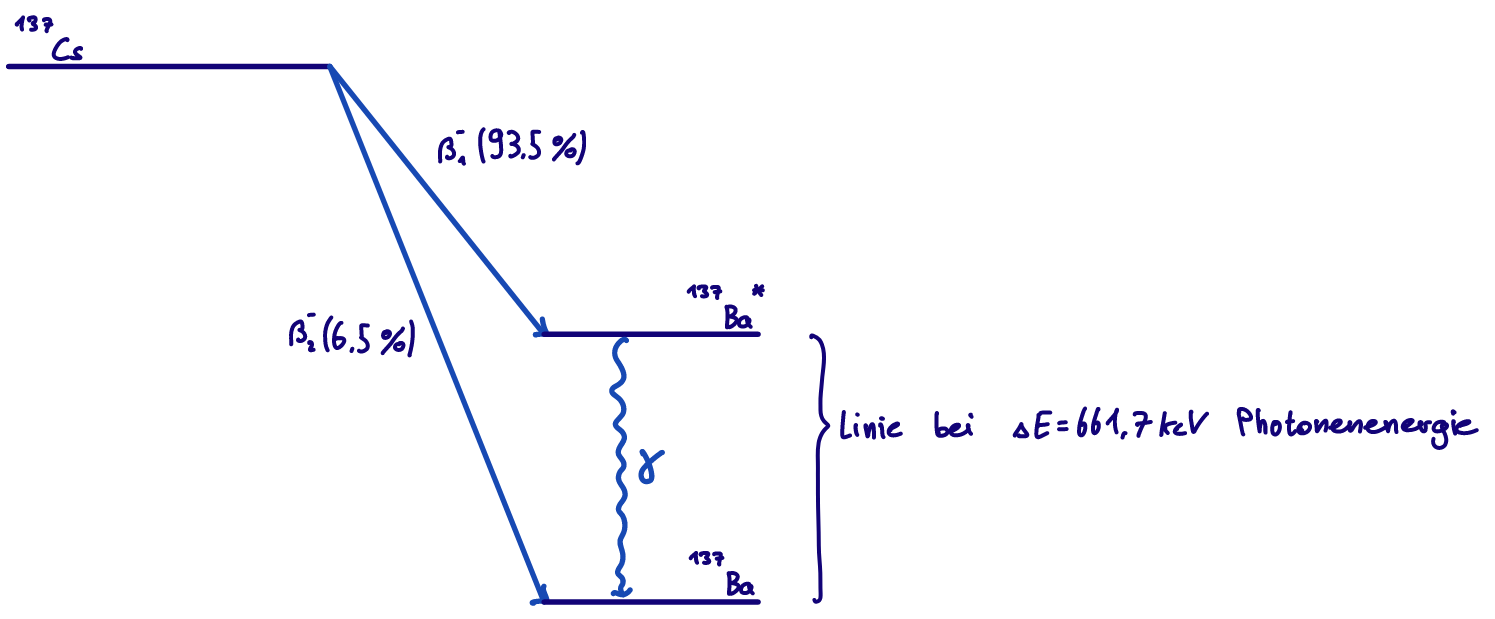
\includegraphics[width = 1\textwidth]{pictures/cs.png}
          \caption{Die möglichen $\beta^-$-Zerfälle von \ce{^{137}Cs} in \ce{^{137}Ba} sowie dessen angeregten Zustand \ce{^{137}Ba}$^*$ und anschließender Übergang in den Grundzustand von \ce{^{137}Ba} unter Aussendung eines Photons. Bearbeitet aus }
          \label{fig:cs_schema}
        \end{figure}
    
        \FloatBarrier
        
        Für den in Abbildung ... skizzierten Zerfall von \ce{^{60}Co} sind Übergänge in zwei verschiedene angeregte Zustände von \ce{^{60}Ni} möglich. Der energetisch höhere Zustand liegt bei 
        \SI{2505.7}{\kilo\electronvolt} und der niedrigere bei \SI{1332.5}{\kilo\electronvolt}. Der energetisch niedrigere Zustand geht direkt in den Grundzustand über und es wird ein Photon mit einer Energie
        von \SI{1332.5}{\kilo\electronvolt} ausgesendet. Die Relaxation des energetisch höheren Zustands findet in zwei Schritten statt. Zunächst geht dieser Zustand in den niederenergetischen angeregten Zustand 
        über, wobei ein Photon mit der Energie \SI{1173.2}{\kilo\electronvolt} ausgesendet wird. Anschließend geht es in den Grundzustand des \ce{^{60}Ni} über. Aufgrund der zwei angeregten Endzustände des 
        $\beta^-$-Zerfalls strahlt eine \ce{^{60}Co}-Quzelle mit zwei charakteristischen Energien.

        \FloatBarrier

        \begin{figure}[h]
          \centering
          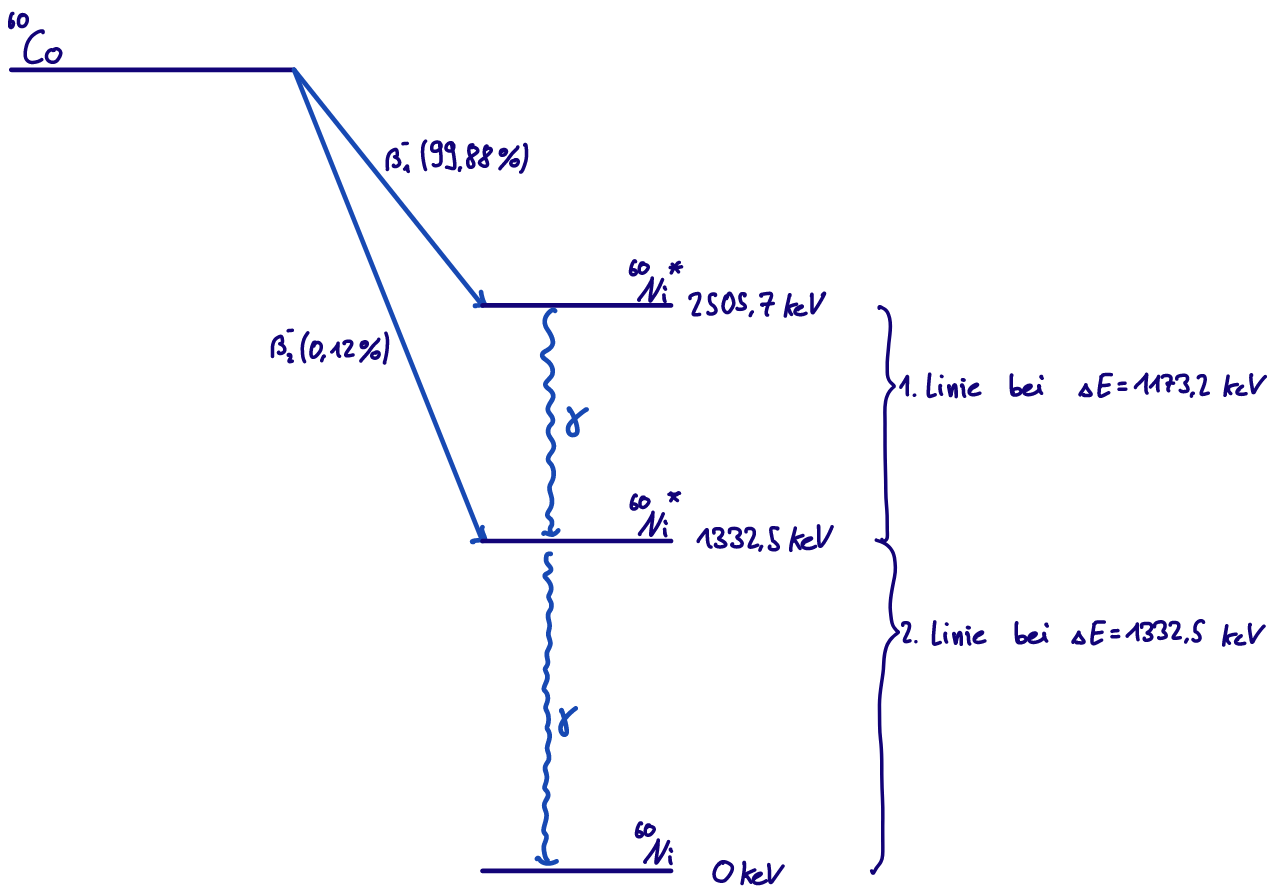
\includegraphics[width = 1\textwidth]{pictures/co.png}
          \caption{Die möglichen $\beta^-$-Zerfälle von \ce{^{60}Co} in die angeregten Zustände von \ce{^{60}Ni} und anschließende Übergänge in den Grundzustand von \ce{^{60}Ba} unter Aussendung zwei Photonen verschiedener Energien. Bearbeitet aus }
          \label{fig:co_schema}
        \end{figure}
    
        \FloatBarrier

